\section{Submodular Orienteering on a Multi-Partite Graph}
\label{sec:path_dependent_optimization}

Using the wingman constraint, we have converted the path-planning problem on a topological graph to a path-planning problem on a multi-partite graph.
Using the observation model and the information measurement we defined, the reward collection can be described by a submodular function $ f() $ [\cite{goodrich2013toward}].
In this section, we will merge these two properties to define a submodular orienteering problem on a multi-partite graph.


\begin{mydef}[\textbf{Submodular Function}][\cite{krause2012submodular}]
\label{def:submod_func}
A submodular function over a set $ V $ is a function  $ f : 2^{V} \rightarrow \mathbb{R} $ that satisfies for every $ A, B \subseteq V $,
\begin{equation}
\label{eq:submod}
f(A \cap B) + f(A \cup B) \leq f(A) + f(B).
\end{equation}
\end{mydef}

A \emph{conditional submodular function} can be similarly defined.

\begin{mydef}[\textbf{Conditional Submodular Function}]
\label{def:cond_submod_func}
A conditional submodular function over a set $ V $ is a function $ f : 2^{V} \times 2^{V} \rightarrow \mathbb{R} $, which is defined for all $ A, B \subseteq V $, 
\begin{equation}
\label{eq:cond_submod}
f( A \mid B ) = f( A \cap B ) - f( B ).
\end{equation}
This function inherits the submodularity, which means that every $ A, B, C \subseteq V $,
\begin{equation}
\label{eq:cond_submod_prop}
f(A \mid B \cup C) \leq f(A \mid B).
\end{equation}

See the proof in Appendix \ref{app:cond_submod_prop}.

\end{mydef}

Without loss of generality, we write $ f( x_{1} , \cdots x_{t} ), x_{1} , \cdots x_{t} \in X $ to indicate that $ f( \{ x_{1} , \cdots x_{t} \}) $.
This notational convenience will also be used for the \emph{conditional submodular function} in equation \eqref{eq:cond_submod}.

%By Lemma \ref{Lemma1}, we have the human's path $ Y^{H} $ known.
%Thus the wingman constraint can be converted into a multi-partite graph like Figure \ref{fig:MultiPartite} in Section \ref{sec:unfold_solution_space}.
By Lemma \ref{Lemma1}, we know that the optimal solution at one time step depends on the solutions chosen at previous time steps. 
In [\cite{krause2012submodular}], it was shown that the entropy and mutual information functions are both submodular.
Thus, the path-dependent optimization problem can be formally defined as a \emph{submodular orienteering on a multi-partite graph}, as follow:

\begin{mydef}[\textbf{Submodular Orienteering on a Multi-Partite Graph}]
\label{def:submod_orienteer}
Given a directed multi-partite graph $ G = (V, E, T) $, each edge $ e \in E $ defines a directed transition from a vertex in partition $ V(t) $ to a vertex in partition $ V(t+1) $, $ t \in [1, T-1] $.
The submodular orienteering problem on a directed multi-partite graph $ G $ is to find a path of length $ T $ that maximizes the total reward collected from a submodular function $ f() $.
\end{mydef}

Without loss of generality, we assume that the optimal search for path planning always starts from same vertex.
Thus, we have only one vertex in partition $ V(1) $, which is shown in Figure \ref{fig:MultiPartite}.
By the submodularity of the conditional mutual information, we can represent $ I(\mathbf{S}; \mathbf{O}^{X} \mid \mathbf{O}^{Y^{h}}) $ by a submodular function  $ f(X) $. 
By Definition \ref{def:submod_orienteer}, we can rewrite equation 
 \eqref{eq:objFunc} as 

\begin{equation}
\label{eq:gnr_obj}
\begin{aligned}
Objective: & X^{*} = \underset{X}{\arg\max} f(X); \\
Constraint: & |X| = T, x_{t} \in V(t), (x_{t}, x_{t+1}) \in E.
\end{aligned}
\end{equation}

Due to Property \ref{prop:orderIndependence}, we write $ f( [x_{1}, x_{2} , \cdots , x_{t} ]^{T} ) $ as $ f(x_{1}, x_{2}, \cdots , x_{t}) $ for simplicity.

By Definition \ref{def:submod_func}, Definition \ref{def:cond_submod_func} and Lemma \ref{Lemma1}, we have
\begin{equation}
\label{eq:gnr_f_chain}
f(x_{1}, x_{2}, \cdots , x_{T}) = f(x_{1}) + f(x_{2} \mid x_{1}) + \cdots + f(x_{T} \mid x_{1}, \cdots , x_{T-1}).
\end{equation}

If we let $ \hat{x}_{t} $ denote the answer to the optimality found at time step $ t $ in considering payoff to arrive and payoff to go,  we can have optimal substructures solved as 
\begin{equation}
\label{eq:max_2}
\hat{x}_{t} = \arg \max_{X_{t}} \left[ f(x_{t} \mid x_{1} , \cdots , x_{t-1})
+ \max_{X_{t+1}, \cdots , X_{T}} f(x_{t+1}, \cdots , x_{T} \mid x_{1}, \cdots , x_{t})
\right].
\end{equation}

$ X_{t} $ is defined by the constraint in equation \eqref{eq:objFunc}, which indicates the search space at time step $ t $.
In order to solve equation \eqref{eq:max_2}, we define the first term as \emph{instant reward} and the second term as \emph{maximum future reward}.

\begin{mydef}[\textbf{Instant Reward}]
\label{def:instant_reward}
Define the instant reward as 
\begin{equation}
\label{eq:def_g}
g(x_{t} \mid x_{1} , \cdots , x_{t-1} ) = f(x_{t} \mid x_{1} , \cdots , x_{t-1}). 
\end{equation}
\end{mydef}

By definition \ref{def:cond_submod_func}, instant reward represents the reward collected by choosing $ x_{t} $ after $ x_{t-1} , \cdots , x_{1} $ have been visited.

\begin{mydef}[\textbf{Maximum Future Reward}]
\label{def:max_future_reward}
Define the maximum future reward as
\begin{equation}
\label{eq:def_h}
h(x_{1} , \cdots, x_{t'} ) = \max_{V(t'+1), \cdots , V(T)} f(x_{t+1}, \cdots x_{T} \mid x_{1}, \cdots , x_{t'}),
\end{equation} 
in the constraint that
\begin{equation}
\label{eq:def_h:constraint1}
\forall \tau \in \{ t'+1 , \cdots , T \},  x_{\tau} \in V(\tau)
\end{equation}
and
\begin{equation}
\label{eq:def_h:constraint2}
\forall \tau \in \{ t'+2, \cdots ,T-1 \}, ( x_{\tau-1}, x_{\tau} ) \in E .
\end{equation}
\end{mydef}

\begin{figure}
\centering
\includegraphics[width=0.5\linewidth]{./images/DefineFuncH.pdf}
\caption{Maximum future reward.}
\label{fig:DefineFuncH}
\end{figure}

The function $ h() $ indicates the maximum future reward of a sub-path that concatenates $ x_{t} $ after $ \{  x_{1} , \cdots, x_{t} \} $ has been visited. 
$  x_{t} $ has the biggest time index in $ \{  x_{1} , \cdots, x_{t-1} , x_{t} \} $.
We would like to figure that in defining the instant reward and the maximum future reward, $ \{  x_{1} , \cdots, x_{t-1} , x_{t} \} $ can be any set of vertices instead of a set of vertices in a sub-path.

Figure \ref{fig:DefineFuncH} gives an example on how $ h(v^{1}_{1}, v^{1}_{2}, v^{2}_{3}, v^{2}_{5}) $ is calculated.
There exists a jump from partition $ V(3) $ to partition $ V(5) $ in calculating $ f() $.
Any vertex in partition $ V(4) $ is skipped.
Since we are calculating the future reward, we only consider the time indices that are bigger than the largest time index in the given sub-path $ \{ v^{1}_{1}, v^{1}_{2}, v^{2}_{3}, v^{2}_{5}  \} $.
In the example that is given in Figure \ref{fig:DefineFuncH}, $ V(6) $ is the only ``future'' partition.

\begin{mydef}[\textbf{Maximum Total Reward}]
\label{def:max_total_reward}
Define the maximum total reward from choosing $ x_{t} $ after $ x_{1} \cdots , x_{t'} $ have been chosen as 
\begin{equation}
\label{eq:def_p_0}
\forall t' > t, 
u(x_{t} \mid x_{1} , \cdots , x_{t'} ) = \max_{V(t+1), \cdots , V(T)} f(x_{t}, \cdots x_{T} \mid x_{1}, \cdots , x_{t'}),
\end{equation}
in the constraint that
\begin{equation}
\label{eq:def_p_0:constraint1}
\forall \tau \in \{ t'+1 , \cdots , T-1 \}, x_{ \tau } \in V( \tau )
\end{equation}
and
\begin{equation}
\label{eq:def_p_0:constraint2}
\forall \tau \in \{ t'+2, \cdots ,T-1 \}, ( x_{ \tau-1 }, x_{ \tau } ) \in E .
\end{equation}
\end{mydef}

It defines that the maximum total reward among all the sub-paths that start from $ x_{t} $ after that $ x_{t'} \cdots , x_{1} $ are visited.

By Definition \ref{def:max_total_reward}, we have
\begin{propty}
\label{prop:u2gh}
\begin{equation}
\label{eq:def_p}
u(x_{t} \mid x_{1} , \cdots , x_{t'} ) = g(x_{t} \mid x_{1} , \cdots , x_{t'} ) + h( x_{1} , \cdots, x_{t'}, x_{t} ).
\end{equation}
\begin{proof}
The proof is given in Appendix \ref{app:proof_prop_u2gh}.
\end{proof}
\end{propty}

Figure \ref{fig:DefineFuncP} gives an example.
After $ v^{1}_{1}, v^{1}_{2} , v^{2}_{3} $ has been visited, the maximum total reward of sub-paths, which starts from $ v^{2}_{5} $, consists of the instant reward $ g( v^{2}_{5} \mid v^{1}_{1}, v^{1}_{2} , v^{2}_{3} ) $ and the maximum future reward $ h( v^{1}_{1}, v^{1}_{2} , v^{2}_{3}, v^{2}_{5} ) $.

By Property \ref{prop:orderIndependence}, we also have
\begin{propty}
\label{prop:u2gh_2}
\begin{equation}
\label{eq:u2gh_2:0}
u( x_{t} \mid x_{1} , \cdots , x_{t'} ) = f( x_{t} \mid \tilde{X}(x_{t}), x_{1} , \cdots , x_{t'} ) +  \max_{x_{t+1} \in V(t+1) \land ( x_{t}, x_{t+1} ) \in E} u( x_{t+1} \mid x_{1} , \cdots , x_{t'} ),
\end{equation}
in which
\begin{equation}
\label{eq:u2gh_2:1}
\tilde{X}(x_{t}) = \arg \max_{ V(t+1) \cdots V(T) } f( x_{t+1} \cdots x_{T} \mid x_{1} , \cdots , x_{t'} )
\end{equation}
in the constraint that
\begin{equation}
\label{eq:u2gh_2:1:constraint}
\forall \tau \in \{ t+1 , \cdots , T \},  x_{ \tau } \in V( \tau ) \land ( x_{ \tau-1 }, x_{ \tau } ) \in E .
\end{equation}
%and
%\begin{equation}
%\tilde{X}(x_{t}) = { \tilde{x}_{t+1}, \cdots \tilde{x}_{T} }.
%\end{equation}
\begin{proof}
The proof is given in Appendix \ref{app:proof_prop_u2gh_2}
\end{proof}
\end{propty}

\begin{figure}
\centering
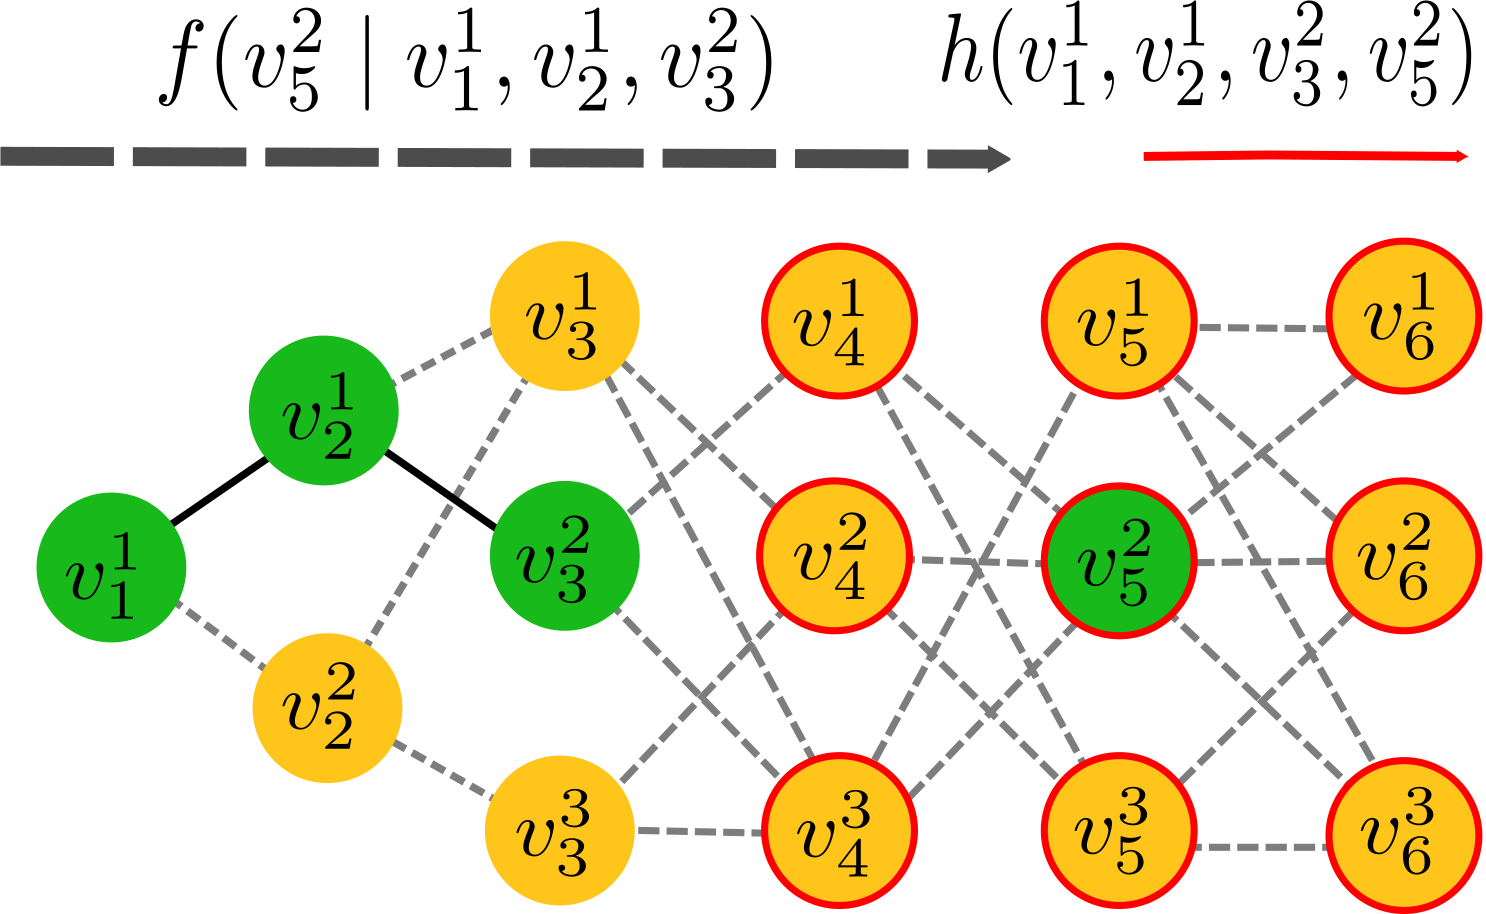
\includegraphics[width=0.5\linewidth]{./images/DefineFuncP.pdf}
\caption{Maximum total reward.}
\label{fig:DefineFuncP}
\end{figure}

By definition of equations \eqref{eq:def_h} and \eqref{eq:def_p}, we have 
\begin{propty}
\label{prop:h2p}
\begin{equation}
\label{eq:h2p}
h( x_{1}, \cdots x_{t'} ) = \max_{x_{t'+1} \in V(t'+1) \land (v_{t'}, x_{t'+1}) \in E} u(x_{t'+1} \mid x_{1}, \cdots x_{t'} ).
\end{equation}
\begin{proof}
The proof is given in Appendix \ref{app:proof_prop_h2p}.
\end{proof}
\end{propty}
After $ x_{t'}, \cdots , x_{1} $ have been visited, there is a vertex $ x^{*}_{t'+1} $ at time $ t' + 1 $ which has the biggest value of maximum total reward in those vertices that are connected with $ x_{t'} $. 
The maximum total reward that is calculated from vertex $ x^{*}_{t'+1} $ with $ x_{1}, \cdots x_{t'} $ visited is equivalent to the maximum future reward of $ x_{t'}, \cdots , x_{1} $.

With defined rewards, we can rewrite equation \eqref{eq:max_2} as
\begin{equation}
\label{eq:max_21}
\hat{x}_{t} = \arg \max_{X_{t}} u(x_{t} \mid x_{1} , \cdots , x_{t-1}).
\end{equation}

%At time $ t $, $ g(x_{t} \mid x_{t-1}, \cdots , x_{1}) $ gives the instant reward of choosing $ x_{t} $ with previous sub-solution $ x_{t-1}, \cdots , x_{1} $ given; $ h(x_{t} , x_{t-1} , \cdots, x_{1} ) $ gives the maximum future reward with choices made from $ 1 $ to $ t $.
If $ u(x_{t} \mid x_{1} , \cdots , x_{t-1}) $ at each step can be calculated correctly at each time step, the solution found can be optimal by Bellmen's \emph{principle of optimality} [\cite{lewis1986optimal}].
Due to the path dependence, calculating future reward at each step is NP-hard.
Brute Force Search exhaustively explores all possible future sub-paths so that it can return the maximum future reward.
Its disadvantage on complexity makes it inapplicable.
Using only a greedy search provides good efficiency but no performance guarantee in this case [\cite{krause2012submodular}], which is discussed in section \ref{sec:related_work}.
Submodularity-based approaches provide useful solutions that have guaranteed performance bounds when sensors/robots can be placed at arbitrary locations, but do not perform well in the presence of path constraints.
In this paper, we import future reward estimation to approximate this optimization calculation process.
